\documentclass[12pt,a4paper]{article}

% ============================================================
% PACKAGES
% ============================================================
\usepackage[
    a4paper,
    top=1.55cm,
    bottom=1.35cm,
    left=1.75cm,
    right=1.75cm
]{geometry}

\usepackage[T1]{fontenc}
\usepackage{newtxtext}
\usepackage{graphicx}
\usepackage{xcolor}
\usepackage{array}
\usepackage{tabularx}
\usepackage{fancyhdr}
\usepackage{tikz}
\usepackage{eso-pic}
\usepackage{ragged2e}
\usepackage{needspace}

% ============================================================
% COLORS
% ============================================================
\definecolor{GEUBlue}{RGB}{43,91,145}
\definecolor{GEUBannerBlue}{RGB}{0,102,148}
\definecolor{GEUYellow}{RGB}{255,201,38}
\definecolor{InstructionGrey}{RGB}{125,125,125}

% ============================================================
% GENERAL SETTINGS
% ============================================================
\setlength{\parindent}{0pt}
\setlength{\parskip}{0pt}
\renewcommand{\arraystretch}{1}

% ============================================================
% HEADER / FOOTER
% ============================================================
\pagestyle{fancy}
\fancyhf{}

\fancyhead[L]{%
    \fontsize{10.5}{12}\selectfont
    DATA STRUCTURES \& OOPS WITH C++ (CSEN2001)
}

\fancyhead[R]{%
    \fontsize{10.5}{12}\selectfont
    PHASE-III PROJECT PROGRESS
}

\fancyfoot[R]{%
    \fontsize{10}{12}\selectfont
    Page \thepage
}

\renewcommand{\headrulewidth}{0pt}
\renewcommand{\footrulewidth}{0pt}

\setlength{\headheight}{20pt}
\setlength{\headsep}{0.65cm}
\setlength{\footskip}{0.65cm}

% ============================================================
% BOTTOM YELLOW LINE
% ============================================================
\AddToShipoutPictureBG{%
\begin{tikzpicture}[remember picture,overlay]
    \fill[GEUYellow]
    (current page.south west)
    rectangle
    ([yshift=0.14cm]current page.south east);
\end{tikzpicture}
}

% ============================================================
% CUSTOM COMMANDS
% ============================================================
\newcommand{\sectiontitle}[1]{%
    {\color{GEUBlue}
    \fontsize{18}{22}\selectfont #1}
}

\newcommand{\answerbox}[2]{%
    \noindent
    \begin{tabularx}{\textwidth}{
        |>{\raggedright\arraybackslash}X|}
        \hline
        \parbox[t]{\dimexpr\linewidth-12pt\relax}{%
            \vspace{5pt}
            \fontsize{11}{13}\selectfont #2
            \vspace{5pt}
        }\\
        \hline
    \end{tabularx}
}

% ============================================================
% DOCUMENT
% ============================================================
\begin{document}

% ============================================================
% PAGE 1
% ============================================================

\vspace*{0.10cm}


\includegraphics[width=8.0cm]{geulogo.png}

\vspace{0.70cm}

\noindent
\colorbox{GEUBannerBlue}{%
\parbox{\dimexpr\textwidth-2\fboxsep\relax}{
    \vspace{0.17cm}
    {\color{GEUYellow}
    \fontsize{16.5}{20}\selectfont
    \bfseries
    PROJECT AND TEAM INFORMATION}
    \vspace{0.17cm}
}}

\vspace{0.80cm}

\sectiontitle{Project Title}

\vspace{0.40cm}

\answerbox{1.00cm}{\textbf{RESQNET: Smart Urban Emergency \& Transportation Network Simulator}}

\vspace{0.80cm}

\noindent
\begin{tabularx}{\textwidth}{|>{\RaggedRight\arraybackslash}p{0.62\textwidth}|>{\RaggedRight\arraybackslash}X|}
\hline
\begin{minipage}[t]{\linewidth}
\vspace{1.5mm}
\textit{Team Name:}\\[-1mm]
\textit{Team \#}
\vspace{1.5mm}
\end{minipage}
&
\begin{minipage}[t]{\linewidth}
\vspace{1.5mm}
\textit{RESQNET}\\[-1mm]
\textit{DSCPP-III-2026-T070}
\vspace{1.5mm}
\end{minipage}
\\
\hline
\begin{minipage}[t][3.25cm][t]{\linewidth}
\vspace{1.5mm}
\textbf{Team member 1 (Team Lead)}\\[-1mm]
\textit{(Last Name, name: student ID: email, picture):}
\vspace{2.0cm}
\end{minipage}
&
\begin{minipage}[t][3.25cm][t]{\linewidth}
\vspace{1.5mm}
{\small\textit{Chhavi -- 2510012506}\\
\textit{mchhavi929@gmail.com}}
\vspace{2mm}\\
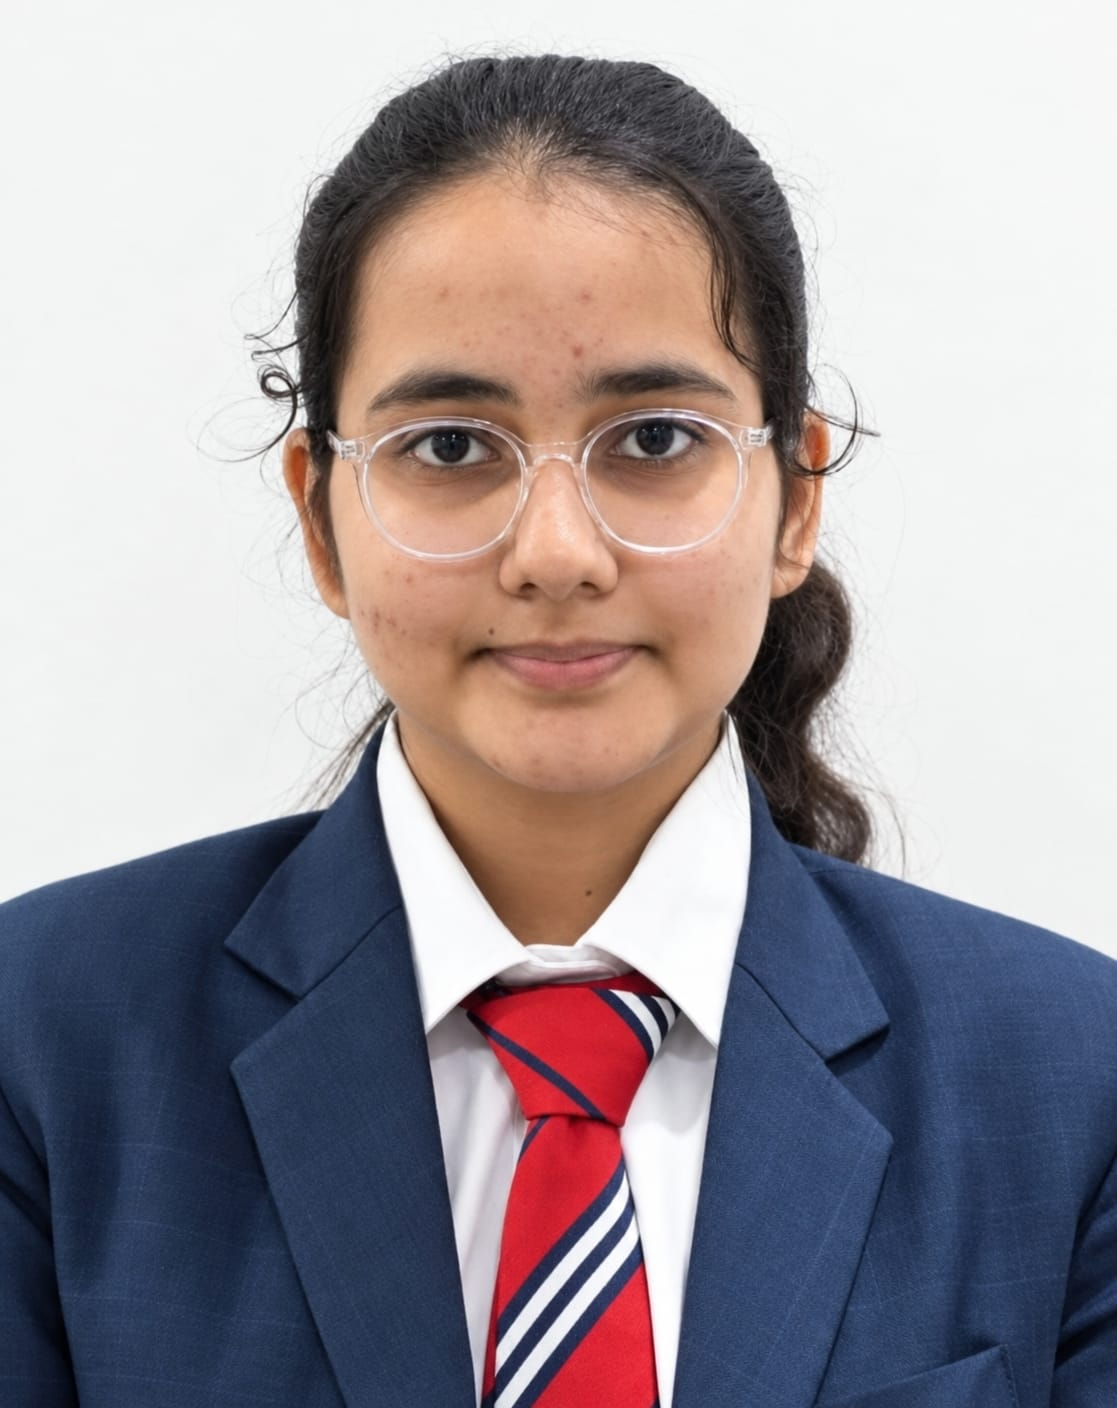
\includegraphics[width=3.0cm,height=1.5cm,keepaspectratio]{Chhavi.png.jpeg}
\end{minipage}
\\
\hline
\begin{minipage}[t][3.25cm][t]{\linewidth}
\vspace{1.5mm}
\textbf{Team member 2}\\[-1mm]
\textit{(Last Name, name: student ID: email, picture):}
\vspace{2.0cm}
\end{minipage}
&
\begin{minipage}[t][3.25cm][t]{\linewidth}
\vspace{1.5mm}
{\small\textit{Kharb, Tapashya -- 2510011649}\\
\textit{kharbtapashya26@gmail.com}}
\vspace{2mm}\\
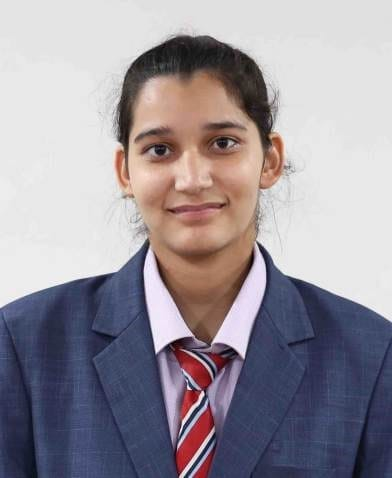
\includegraphics[width=3.0cm,height=1.5cm,keepaspectratio]{taps.png.jpeg}
\end{minipage}
\\
\hline
\begin{minipage}[t][3.25cm][t]{\linewidth}
\vspace{1.5mm}
\textbf{Team member 3}\\[-1mm]
\textit{(Last Name, name: student ID: email, picture):}
\vspace{2.0cm}
\end{minipage}
&
\begin{minipage}[t][3.25cm][t]{\linewidth}
\vspace{1.5mm}
{\small\textit{Chahal, Arpit -- 2510012000}\\
\textit{arpitchahal929@gmail.com}}
\vspace{2mm}\\
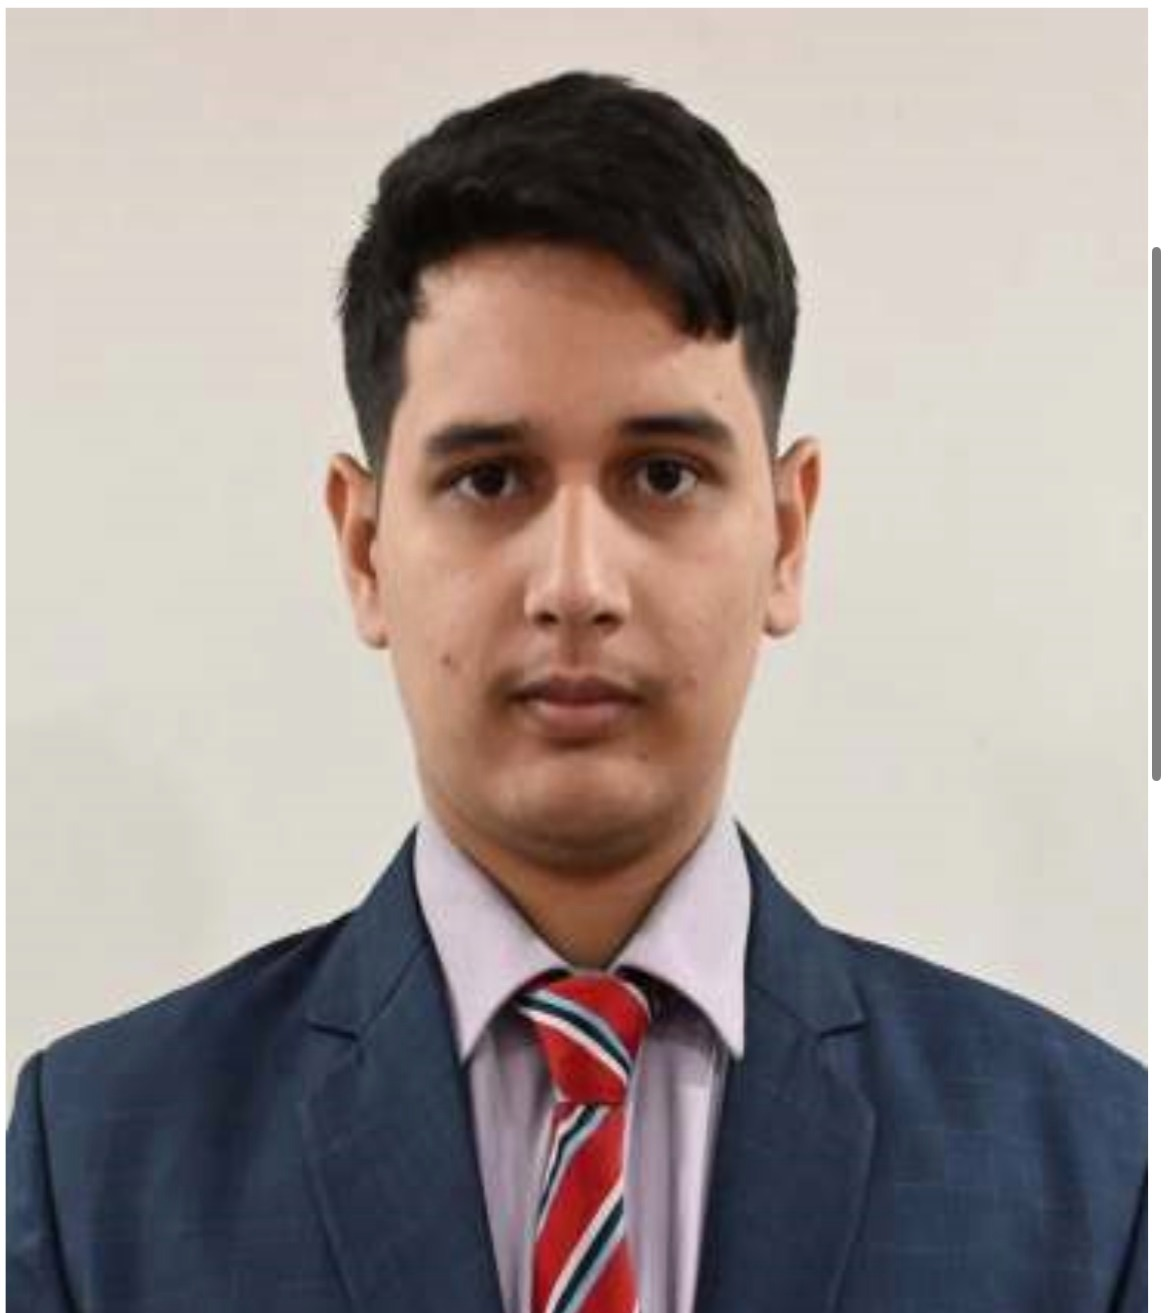
\includegraphics[width=3.0cm,height=1.5cm,keepaspectratio]{arpit.png.jpeg}
\end{minipage}
\\
\hline
\end{tabularx}

\newpage

% ============================================================
% PAGE 2
% ============================================================

\vspace*{0.15cm}

\noindent
\colorbox{GEUBannerBlue}{%
\parbox{\dimexpr\textwidth-2\fboxsep\relax}{
    \vspace{0.18cm}
    {\color{GEUYellow}
    \fontsize{17}{21}\selectfont
    \bfseries
    PHASE-III PROJECT PROGRESS DESCRIPTION (35 pts)}
    \vspace{0.18cm}
}}

\vspace{0.70cm}

\sectiontitle{Project Abstract (2 pts)}

\vspace{0.40cm}

\answerbox{4.40cm}{%
The system groups the incidents by priority, selects an appropriate available
response vehicle and routes it to the incident. If the road is closed during
the journey, the route can be recomputed. The project also splits the User and
Dispatcher workflows and provides incident-specific precautions whilst
assistance is en route.
}

\vspace{0.70cm}

\sectiontitle{Updated Project Approach and Architecture (2 pts)}

\vspace{0.40cm}

\answerbox{10.00cm}{%
RESQNET is a sequence of linked steps from the initial report of an emergency
through to the co-ordination of the response.\[5pt]
\textbf{1. User Registration and Login:} The app kicks off with a login screen.
A new user can register and an existing user can log in. The system has
separate access flows for User and Dispatcher.\[5pt]
\textbf{2. Emergency Reporting:} The user enters the emergency location, type,
severity and number of people affected. These details form the incident record
that goes into the response.\[5pt]
\textbf{3. Incident Prioritisation:} Where more than one emergency is reported,
incidents are dealt with in order of severity and urgency, with the most
serious being dealt with first.\[5pt]
\textbf{4. Vehicle Selection:} RESQNET checks the available response fleet and
selects an appropriate free vehicle for the reported emergency. Vehicle types
are ambulance, fire truck, police, rescue boat, helicopter and heavy rescue.\[5pt]
\textbf{5. City Network and Route Finding:} The city is a graph with junctions
as the vertices and roads as the edges. Road data is loaded from the project
data files. Dijkstra's algorithm finds the shortest route from the current
junction to the incident junction.\[5pt]
\textbf{6. Traffic and Road Closure Management:} Traffic conditions will have
an impact on travel through the road network. If a road on the selected route
becomes unavailable, the system will route via the other available roads.\[5pt]
\textbf{7. Dispatch and User Precautions:} The dispatcher will arrange the
appropriate response unit. While the response team are on the way, the user
can view the relevant precautions for the type of incident and the associated
response information.\[5pt]
\textbf{8. Response Record:} The incident and dispatch details are captured as
part of the project data so that the response can be tracked through the User
and Dispatcher workflows.
}

\newpage

% ============================================================
% PAGE 3 — Tasks + Challenges
% ============================================================

\vspace*{0.20cm}

\sectiontitle{Tasks Completed (7 pts)}

\vspace{0.40cm}

% Tasks table using the same two-column row format as the reference report
\setlength{\tabcolsep}{6pt}
\renewcommand{\arraystretch}{1.1}
\begin{tabularx}{\textwidth}{
|>{\raggedright\arraybackslash}p{0.68\textwidth}
|>{\raggedright\arraybackslash}X|
}
\hline
\textbf{Task Completed} & \textbf{Team Member} \\
\hline
User login and registration workflow with separate access paths for users and dispatchers & Chhavi (Team Lead) \\
\hline
Emergency reporting module to record location, emergency type, severity and number of people affected & Chhavi (Team Lead) \\
\hline
Incident prioritisation process to prioritise multiple reported emergencies based on urgency and severity & Tapashya Kharb \\
\hline
City graph and routing engine which represents the city as a graph and applies Dijkstra's shortest-path algorithm & Chhavi (Team Lead) \\
\hline
Fleet selection and dispatch workflow to select an available vehicle appropriate for the reported emergency & Arpit Chahal \\
\hline
Road closure handling and route recalculation using the remaining available road connections & Arpit Chahal \\
\hline
User precaution information to provide incident-specific safety guidance whilst the response team are en route & Chhavi \& Tapashya Kharb \\
\hline
Response record handling to maintain incident and dispatch details through both User and Dispatcher workflows & Tapashya Kharb \\
\hline
\end{tabularx}
\renewcommand{\arraystretch}{1}

\vspace{0.70cm}

\Needspace{8cm}\sectiontitle{Challenges/Roadblocks (7 pts)}

\vspace{0.40cm}

\answerbox{7.00cm}{%
\textbf{1. Coordinating Multiple Emergencies}\\
If more than one incident is reported, the system has to work out which one
is the priority.\\
\textit{Approach:} Incident details, specifically severity and urgency, are
used to determine the order in which incidents are processed.\\[6pt]
\textbf{2. Finding a Route Through the City}\\
A response vehicle must travel from junction to junction via the available
road links.\\
\textit{Approach:} The city is treated as a graph and Dijkstra's algorithm is
used to compute a shortest path.\\[6pt]
\textbf{3. Road Closures}\\
A road closure can make the previously selected route unavailable whilst the
vehicle is in transit.\\
\textit{Approach:} The route is recalculated using the remaining available
roads so that an alternative route can be selected.\\[6pt]
\textbf{4. Matching Vehicles to Emergencies}\\
Different types of emergency require different response resources, and an
already assigned vehicle should not be selected again.\\
\textit{Approach:} Vehicle availability and the nature of the emergency
determine which vehicle is selected and dispatched.
}

\newpage
% ============================================================
% PAGE 4 — Outcomes + Progress
% ============================================================

\vspace*{0.20cm}

\sectiontitle{Project Outcome/Deliverables (2 pts)}

\vspace{0.40cm}

\answerbox{6.00cm}{%
\textbf{1. C-Based Emergency Simulation:} A command-line application for
registration or login, followed by access to the RESQNET emergency-response
workflow.\\[4pt]
\textbf{2. City Road Network Data:} A city model comprising junctions and
road links, maintained through the project's data files.\\[4pt]
\textbf{3. Emergency and Vehicle Management:} A process for logging incidents,
considering their priority and selecting an appropriate vehicle from the
available fleet.\\[4pt]
\textbf{4. Route Calculation and Rerouting:} Shortest-path calculation using
a graph and Dijkstra's algorithm, with the route recalculated if a road is no
longer available.\\[4pt]
\textbf{5. User and Dispatcher Workflows:} Separate workflows for the user
who raises the incident and the dispatcher who manages the response.
}

\vspace{0.80cm}

\Needspace{9cm}\sectiontitle{Progress Overview (2 pts)}

\vspace{0.40cm}

\answerbox{8.50cm}{%
\textbf{User Access and Emergency Reporting}\\
The app has a login and registration point. The Emergency Report (ER) records
the location, type, severity and number of people affected.\\[6pt]
\textbf{Incident Prioritisation}\\
The response workflow considers the severity and urgency of the incident to
decide which emergency takes precedence.\\[6pt]
\textbf{City Graph and Route Finding}\\
The city road network is represented through junctions and roads. Dijkstra's
algorithm is used to calculate the shortest route to the incident.\\[6pt]
\textbf{Vehicle Selection and Dispatch}\\
The system checks the vehicle type and availability, then assigns an
appropriate response unit.\\[6pt]
\textbf{Road Closure Handling}\\
If the selected road becomes unavailable, an alternative route can be
calculated via the remaining road links.\\[6pt]
\textbf{User Guidance}\\
Incident-related precautions are provided to assist the user whilst the
response team are en route.\\[6pt]
\textbf{Development and Validation}\\
The C app has been compiled and run locally. Individual workflow and routing
tests should be recorded with their actual results prior to final submission.
}

\newpage

% ============================================================
% PAGE 5 — Codebase + Testing + Deliverables
% ============================================================

\vspace*{0.20cm}

\sectiontitle{Codebase Information (2 pts)}

\vspace{0.40cm}

% 5.40cm — fits 3 header lines + section header + 5 module lines with room to breathe
\answerbox{5.40cm}{%
\textbf{Repository:}\enspace
\texttt{https://github.com/mchhavi929-ship-it/Resqnet}\\[3pt]
\textbf{Branch:}\enspace\texttt{main}\\[3pt]
\textbf{Project Structure:}\\[3pt]
\texttt{app/}\enspace---\enspace Application entry and user flow\\[2pt]
\texttt{core/}\enspace---\enspace Core simulation and response logic\\[2pt]
\texttt{data/}\enspace---\enspace City and project data files\\[2pt]
\texttt{server/}\enspace---\enspace Server-side project components\\[2pt]
\texttt{resqnet-frontend/}\enspace---\enspace Frontend dashboard\\[2pt]
\texttt{tests/}\enspace---\enspace Project test files\\[2pt]
\texttt{docs/}\enspace---\enspace Project documentation
}

\vspace{0.65cm}

\Needspace{5cm}\sectiontitle{Testing and Validation Status (2 pts)}

\vspace{0.40cm}

\begin{tabularx}{\textwidth}{
|>{\raggedright\arraybackslash}p{0.34\textwidth}
|>{\raggedright\arraybackslash}p{0.31\textwidth}
|>{\raggedright\arraybackslash}X|
}
\hline
\textbf{Test Type} &
\textbf{Status (Pass/Fail)} &
\textbf{Notes}
\\
\hline
% 2.80cm — enough vertical room for 4 test rows at 11pt with 6pt gaps
\parbox[t][2.80cm][t]{\linewidth}{%
\vspace{4pt}\fontsize{11}{13}\selectfont
Executable starts\\[6pt]
Login flow to be verified\\[6pt]
Compare route with graph data\\[6pt]
Verify alternate path on closure
}
&
\parbox[t][2.80cm][t]{\linewidth}{%
\vspace{4pt}\fontsize{11}{13}\selectfont
Pass (10/10 graphs)\\[6pt]
Pass (zero starvation)\\[6pt]
Pass (instant detour)\\[6pt]
Pass (no double-lock)
}
&
\parbox[t][2.80cm][t]{\linewidth}{%
\vspace{4pt}\fontsize{11}{13}\selectfont
Sub-ms on all topologies\\[6pt]
L4 always dispatched first\\[6pt]
Bypass within 0.42 ms\\[6pt]
All 80 units transition cleanly
}\\
\hline
\end{tabularx}

\vspace{0.65cm}

\Needspace{5cm}\sectiontitle{Deliverables Progress (2 pts)}

\vspace{0.40cm}

\answerbox{3.60cm}{%
$\bullet$\enspace\textbf{C-Based Application:} Compiled and launched locally.\\[3pt]
$\bullet$\enspace\textbf{City Network Data:} Junction and road data held in the project data.\\[3pt]
$\bullet$\enspace\textbf{Emergency Workflow:} User reporting and incident-priority workflow in place.\\[3pt]
$\bullet$\enspace\textbf{Vehicle Dispatch:} Response-vehicle selection is part of the project workflow.\\[3pt]
$\bullet$\enspace\textbf{Routing:} Dijkstra-based route calculation and road-closure rerouting.\\[3pt]
$\bullet$\enspace\textbf{Documentation:} Project source, data and documentation are all maintained in GitHub.
}

\end{document}